\documentclass[]{tufte-handout}

% ams
\usepackage{amssymb,amsmath}

\usepackage{ifxetex,ifluatex}
\usepackage{fixltx2e} % provides \textsubscript
\ifnum 0\ifxetex 1\fi\ifluatex 1\fi=0 % if pdftex
  \usepackage[T1]{fontenc}
  \usepackage[utf8]{inputenc}
\else % if luatex or xelatex
  \makeatletter
  \@ifpackageloaded{fontspec}{}{\usepackage{fontspec}}
  \makeatother
  \defaultfontfeatures{Ligatures=TeX,Scale=MatchLowercase}
  \makeatletter
  \@ifpackageloaded{soul}{
     \renewcommand\allcapsspacing[1]{{\addfontfeature{LetterSpace=15}#1}}
     \renewcommand\smallcapsspacing[1]{{\addfontfeature{LetterSpace=10}#1}}
   }{}
  \makeatother

\fi

% graphix
\usepackage{graphicx}
\setkeys{Gin}{width=\linewidth,totalheight=\textheight,keepaspectratio}

% booktabs
\usepackage{booktabs}

% url
\usepackage{url}

% hyperref
\usepackage{hyperref}

% units.
\usepackage{units}


\setcounter{secnumdepth}{-1}

% citations
\usepackage{natbib}
\bibliographystyle{plainnat}

% pandoc syntax highlighting
\usepackage{color}
\usepackage{fancyvrb}
\newcommand{\VerbBar}{|}
\newcommand{\VERB}{\Verb[commandchars=\\\{\}]}
\DefineVerbatimEnvironment{Highlighting}{Verbatim}{commandchars=\\\{\}}
% Add ',fontsize=\small' for more characters per line
\newenvironment{Shaded}{}{}
\newcommand{\AlertTok}[1]{\textcolor[rgb]{1.00,0.00,0.00}{\textbf{#1}}}
\newcommand{\AnnotationTok}[1]{\textcolor[rgb]{0.38,0.63,0.69}{\textbf{\textit{#1}}}}
\newcommand{\AttributeTok}[1]{\textcolor[rgb]{0.49,0.56,0.16}{#1}}
\newcommand{\BaseNTok}[1]{\textcolor[rgb]{0.25,0.63,0.44}{#1}}
\newcommand{\BuiltInTok}[1]{#1}
\newcommand{\CharTok}[1]{\textcolor[rgb]{0.25,0.44,0.63}{#1}}
\newcommand{\CommentTok}[1]{\textcolor[rgb]{0.38,0.63,0.69}{\textit{#1}}}
\newcommand{\CommentVarTok}[1]{\textcolor[rgb]{0.38,0.63,0.69}{\textbf{\textit{#1}}}}
\newcommand{\ConstantTok}[1]{\textcolor[rgb]{0.53,0.00,0.00}{#1}}
\newcommand{\ControlFlowTok}[1]{\textcolor[rgb]{0.00,0.44,0.13}{\textbf{#1}}}
\newcommand{\DataTypeTok}[1]{\textcolor[rgb]{0.56,0.13,0.00}{#1}}
\newcommand{\DecValTok}[1]{\textcolor[rgb]{0.25,0.63,0.44}{#1}}
\newcommand{\DocumentationTok}[1]{\textcolor[rgb]{0.73,0.13,0.13}{\textit{#1}}}
\newcommand{\ErrorTok}[1]{\textcolor[rgb]{1.00,0.00,0.00}{\textbf{#1}}}
\newcommand{\ExtensionTok}[1]{#1}
\newcommand{\FloatTok}[1]{\textcolor[rgb]{0.25,0.63,0.44}{#1}}
\newcommand{\FunctionTok}[1]{\textcolor[rgb]{0.02,0.16,0.49}{#1}}
\newcommand{\ImportTok}[1]{#1}
\newcommand{\InformationTok}[1]{\textcolor[rgb]{0.38,0.63,0.69}{\textbf{\textit{#1}}}}
\newcommand{\KeywordTok}[1]{\textcolor[rgb]{0.00,0.44,0.13}{\textbf{#1}}}
\newcommand{\NormalTok}[1]{#1}
\newcommand{\OperatorTok}[1]{\textcolor[rgb]{0.40,0.40,0.40}{#1}}
\newcommand{\OtherTok}[1]{\textcolor[rgb]{0.00,0.44,0.13}{#1}}
\newcommand{\PreprocessorTok}[1]{\textcolor[rgb]{0.74,0.48,0.00}{#1}}
\newcommand{\RegionMarkerTok}[1]{#1}
\newcommand{\SpecialCharTok}[1]{\textcolor[rgb]{0.25,0.44,0.63}{#1}}
\newcommand{\SpecialStringTok}[1]{\textcolor[rgb]{0.73,0.40,0.53}{#1}}
\newcommand{\StringTok}[1]{\textcolor[rgb]{0.25,0.44,0.63}{#1}}
\newcommand{\VariableTok}[1]{\textcolor[rgb]{0.10,0.09,0.49}{#1}}
\newcommand{\VerbatimStringTok}[1]{\textcolor[rgb]{0.25,0.44,0.63}{#1}}
\newcommand{\WarningTok}[1]{\textcolor[rgb]{0.38,0.63,0.69}{\textbf{\textit{#1}}}}

% longtable

% multiplecol
\usepackage{multicol}

% strikeout
\usepackage[normalem]{ulem}

% morefloats
\usepackage{morefloats}


% tightlist macro required by pandoc >= 1.14
\providecommand{\tightlist}{%
  \setlength{\itemsep}{0pt}\setlength{\parskip}{0pt}}

% title / author / date
\title{Try Bayesian Survival Analysis using the JACC study data (Bayesian
Survival Analysis presentations)}
\author{Chaochen Wang \textbar{} Aichi Medical University}
\date{2020-01-12}

\usepackage{booktabs}
\usepackage{longtable}
\usepackage{array}
\usepackage{multirow}
\usepackage{wrapfig}
\usepackage{float}
\usepackage{colortbl}
\usepackage{pdflscape}
\usepackage{tabu}
\usepackage{threeparttable}
\usepackage{threeparttablex}
\usepackage[normalem]{ulem}
\usepackage{makecell}
\usepackage{xcolor}

\begin{document}

\maketitle




\hypertarget{parametric-survival-analysis-model-in-a-bayesian-way}{%
\subsection{Parametric Survival Analysis Model (in a Bayesian
way)}\label{parametric-survival-analysis-model-in-a-bayesian-way}}

\begin{marginfigure}
Weibull Survival funciton in a proportional hazard way expression is:
\[S(t | \mathbf{x}) = \exp\{ -\lambda t ^\kappa e^{\mathbf{\beta_{PH}^T x}} \}\]
\end{marginfigure}

\begin{marginfigure}
Weibull Survival funciton in a AFT way expression is:
\[S(t | \mathbf{x}) = \exp\{ -\lambda t ^\kappa e^{\kappa\mathbf{\beta_{AFT}^T x}} \}\]
\end{marginfigure}

\begin{itemize}
\item
  We chose Weibull model to describe the survival data we have.
\item
  Weibull model is both a proportional hazard model and a accelerated
  failure time (AFT) model. The relationship between the acceleration
  factor and log hazard ratio:
\end{itemize}

\[
\exp(\beta^T_{PH}) = \exp(\kappa\beta^T_{AFT})
\]

\hypertarget{an-example-of-a-crude-weibull-model-using-the-jags-program-in-r}{%
\subsection{An example of a crude Weibull model using the JAGS program
in
R:}\label{an-example-of-a-crude-weibull-model-using-the-jags-program-in-r}}

\begin{Shaded}
\begin{Highlighting}[]
\NormalTok{jacc.weibull.model <-}\StringTok{ }\ControlFlowTok{function}\NormalTok{() \{}
  \ControlFlowTok{for}\NormalTok{(i }\ControlFlowTok{in} \DecValTok{1}\OperatorTok{:}\DecValTok{39386}\NormalTok{)\{}
    \CommentTok{# sAge[i] <- (Age[i] - mean(Age[])) / sd(Age[])}
\NormalTok{    is.censored[i] }\OperatorTok{~}\StringTok{ }\KeywordTok{dinterval}\NormalTok{(t[i], c[i])}
\NormalTok{    t[i] }\OperatorTok{~}\StringTok{ }\KeywordTok{dweib}\NormalTok{(shape, lambda[i])}
\NormalTok{    lambda[i] <-}\StringTok{ }\KeywordTok{exp}\NormalTok{(}\OperatorTok{-}\NormalTok{mu[i] }\OperatorTok{*}\StringTok{ }\NormalTok{shape)}
\NormalTok{    mu[i] <-}\StringTok{ }\NormalTok{beta[}\DecValTok{1}\NormalTok{] }\OperatorTok{+}\StringTok{ }\NormalTok{beta[}\DecValTok{2}\NormalTok{]}\OperatorTok{*}\KeywordTok{equals}\NormalTok{(Mlkfre[i], }\DecValTok{2}\NormalTok{) }\OperatorTok{+}
\StringTok{      }\NormalTok{beta[}\DecValTok{3}\NormalTok{]}\OperatorTok{*}\KeywordTok{equals}\NormalTok{(Mlkfre[i], }\DecValTok{3}\NormalTok{) }\OperatorTok{+}\StringTok{ }\NormalTok{beta[}\DecValTok{4}\NormalTok{] }\OperatorTok{*}\StringTok{ }\KeywordTok{equals}\NormalTok{(Mlkfre[i], }\DecValTok{4}\NormalTok{) }\OperatorTok{+}
\StringTok{      }\NormalTok{beta[}\DecValTok{5}\NormalTok{] }\OperatorTok{*}\StringTok{ }\KeywordTok{equals}\NormalTok{(Mlkfre[i], }\DecValTok{5}\NormalTok{) }\CommentTok{# + }
      \CommentTok{# beta[6] * sAge[i]}
    
    \CommentTok{### calculate log-likelihoods}
    \CommentTok{# y[i] <- ifelse(is.censored[i], c[i], t[i])}
    \CommentTok{# loglik[i] <- log(ifelse(is.censored[i],}
    \CommentTok{#                  exp(-lambda[i] * (y[i] ^ shape)),}
    \CommentTok{#               shape * lambda[i] * (y[i] ^ (shape - 1)) * exp(-lambda[i] * (y[i] ^ shape))))}
\NormalTok{  \}}
  
  \CommentTok{## priors for betas}
  \ControlFlowTok{for}\NormalTok{(j }\ControlFlowTok{in} \DecValTok{1}\OperatorTok{:}\DecValTok{5}\NormalTok{)\{}
\NormalTok{    beta[j] }\OperatorTok{~}\StringTok{ }\KeywordTok{dnorm}\NormalTok{(}\DecValTok{0}\NormalTok{, }\FloatTok{0.001}\NormalTok{)}
\NormalTok{  \}}
  
  \CommentTok{### prior for shape}
\NormalTok{  shape }\OperatorTok{~}\StringTok{ }\KeywordTok{dgamma}\NormalTok{(.}\DecValTok{001}\NormalTok{, }\FloatTok{.001}\NormalTok{)}
  
  \CommentTok{### Generated values}
\NormalTok{  AFT[}\DecValTok{2}\NormalTok{] <-}\StringTok{ }\KeywordTok{exp}\NormalTok{(beta[}\DecValTok{2}\NormalTok{])}
\NormalTok{  HR[}\DecValTok{2}\NormalTok{] <-}\StringTok{ }\KeywordTok{exp}\NormalTok{(shape }\OperatorTok{*}\StringTok{ }\NormalTok{beta[}\DecValTok{2}\NormalTok{])}
\NormalTok{  p.crit[}\DecValTok{2}\NormalTok{] <-}\StringTok{ }\KeywordTok{step}\NormalTok{(}\DecValTok{1} \OperatorTok{-}\StringTok{ }\NormalTok{HR[}\DecValTok{2}\NormalTok{])}
  
\NormalTok{  AFT[}\DecValTok{3}\NormalTok{] <-}\StringTok{ }\KeywordTok{exp}\NormalTok{(beta[}\DecValTok{3}\NormalTok{])}
\NormalTok{  HR[}\DecValTok{3}\NormalTok{] <-}\StringTok{ }\KeywordTok{exp}\NormalTok{(shape }\OperatorTok{*}\StringTok{ }\NormalTok{beta[}\DecValTok{3}\NormalTok{])}
\NormalTok{  p.crit[}\DecValTok{3}\NormalTok{] <-}\StringTok{ }\KeywordTok{step}\NormalTok{(}\DecValTok{1} \OperatorTok{-}\StringTok{ }\NormalTok{HR[}\DecValTok{3}\NormalTok{])}
  
\NormalTok{  AFT[}\DecValTok{4}\NormalTok{] <-}\StringTok{ }\KeywordTok{exp}\NormalTok{(beta[}\DecValTok{4}\NormalTok{])}
\NormalTok{  HR[}\DecValTok{4}\NormalTok{] <-}\StringTok{ }\KeywordTok{exp}\NormalTok{(shape }\OperatorTok{*}\StringTok{ }\NormalTok{beta[}\DecValTok{4}\NormalTok{])}
\NormalTok{  p.crit[}\DecValTok{4}\NormalTok{] <-}\StringTok{ }\KeywordTok{step}\NormalTok{(}\DecValTok{1} \OperatorTok{-}\StringTok{ }\NormalTok{HR[}\DecValTok{4}\NormalTok{])}
  
\NormalTok{  AFT[}\DecValTok{5}\NormalTok{] <-}\StringTok{ }\KeywordTok{exp}\NormalTok{(beta[}\DecValTok{5}\NormalTok{])}
\NormalTok{  HR[}\DecValTok{5}\NormalTok{] <-}\StringTok{ }\KeywordTok{exp}\NormalTok{(shape }\OperatorTok{*}\StringTok{ }\NormalTok{beta[}\DecValTok{5}\NormalTok{])}
\NormalTok{  p.crit[}\DecValTok{5}\NormalTok{] <-}\StringTok{ }\KeywordTok{step}\NormalTok{(}\DecValTok{1} \OperatorTok{-}\StringTok{ }\NormalTok{HR[}\DecValTok{5}\NormalTok{])}
\NormalTok{\}}
\end{Highlighting}
\end{Shaded}

You can use the following codes to run the above model (careful about
the cost of time):

\begin{Shaded}
\begin{Highlighting}[]
\KeywordTok{library}\NormalTok{(R2jags) }\CommentTok{#conect to jags sampling engine in R}
\NormalTok{jagsfit <-}\StringTok{ }\KeywordTok{jags.parallel}\NormalTok{(}\DataTypeTok{data =}\NormalTok{ JACCdata,}
                         \DataTypeTok{parameters.to.save =} \KeywordTok{c}\NormalTok{(}\StringTok{"beta[5]"}\NormalTok{, }\StringTok{"HR[5]"}\NormalTok{, }\StringTok{"AFT[5]"}\NormalTok{),}
                         \CommentTok{#add more variables if you want to check more}
                         \DataTypeTok{n.iter =} \DecValTok{10000}\NormalTok{, }
                         \DataTypeTok{n.burnin =} \DecValTok{2500}\NormalTok{, }
                         \DataTypeTok{n.chains =} \DecValTok{3}\NormalTok{,}
                         \DataTypeTok{model.file =}\NormalTok{ jacc.weibull.model)}
\end{Highlighting}
\end{Shaded}

\hypertarget{check-model-fitting}{%
\subsection{Check model fitting:}\label{check-model-fitting}}

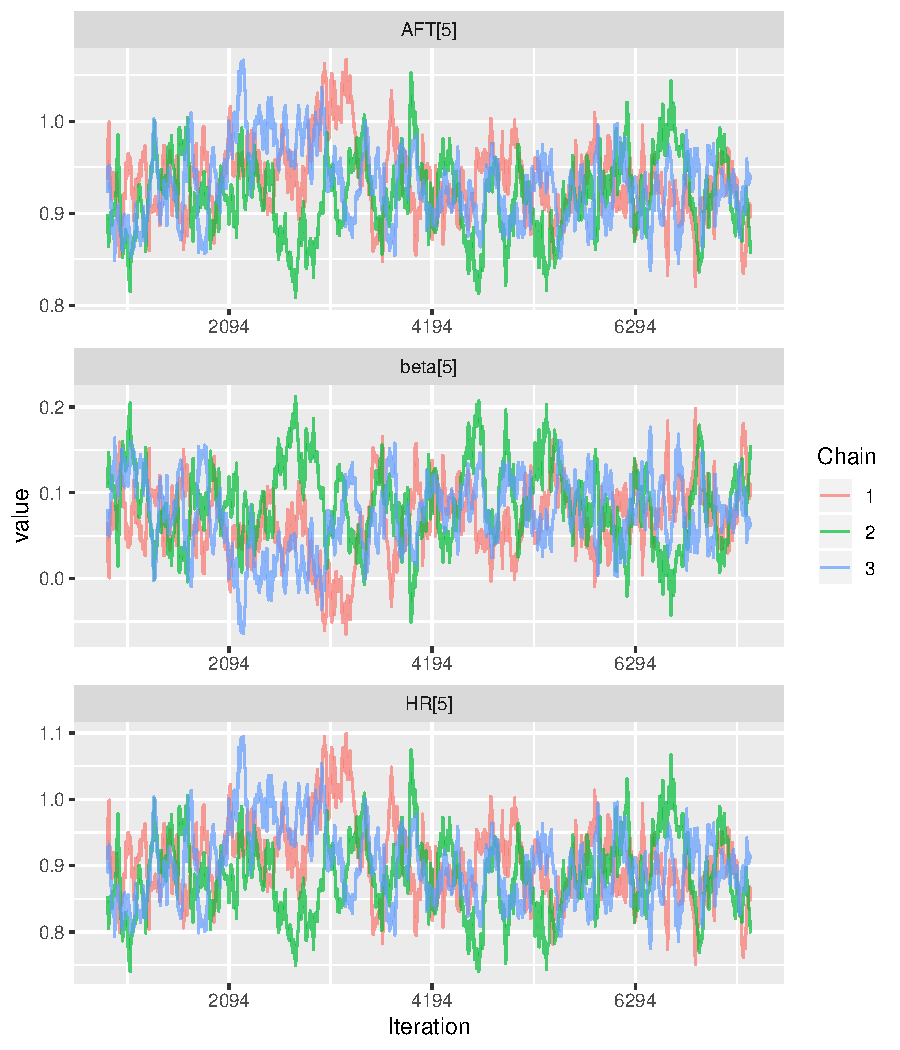
\includegraphics{HandOutEngBayes_files/figure-latex/unnamed-chunk-5-1}

\bibliography{skeleton.bib}



\end{document}
